\begin{figure}
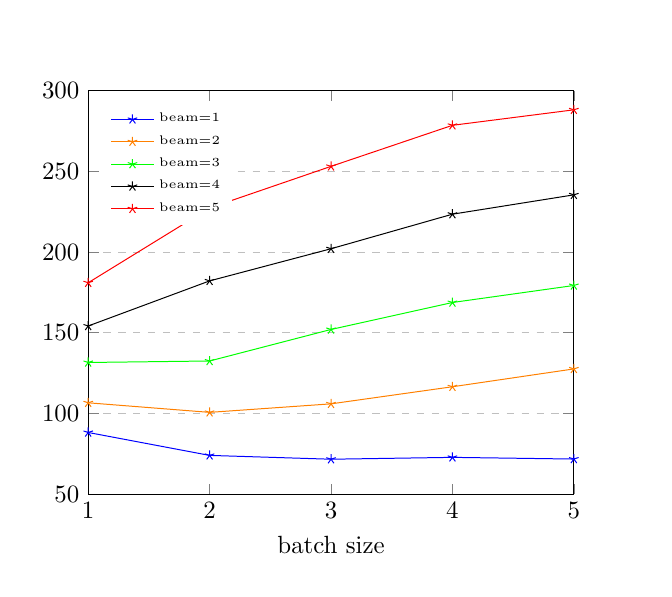
\begin{tikzpicture}
\scalebox{0.9}{
\begin{axis}[
    %title={CPU time},
    xlabel={batch size},
    %ylabel={},
    xmin=1, xmax=5,
    ymin=50, ymax=300,
    xtick={1,2,3,4,5},
    ytick={50,100,150,200,250,300},
    legend pos=north west,
    %legend style={font=\fontsize{4}{5}\selectfont},
    legend style={font=\tiny, draw=none},
    ymajorgrids=true,
    grid style=dashed,
]
 
\addplot[
    color=blue,
    mark=star,
    ]
    coordinates {
    (1,88.2)	(2,74)	(3,71.63)	(4,72.78)	(5,71.74)
    };

\addplot[
    color=orange,
    mark=star,
    ]
    coordinates {
    (1,106.59)	(2,100.66)	(3,105.94)	(4,116.53)	(5,127.58)
    };
    
\addplot[
    color=green,
    mark=star,
    ]
    coordinates {
    (1,131.57)	(2,132.49)	(3,152.02)	(4,168.73)	(5,179.27)
    };

\addplot[
    color=black,
    mark=star,
    ]
    coordinates {
    (1,154.18)	(2,182.12)	(3,202.04)	(4,223.45)	(5,235.43)
    };

\addplot[
    color=red,
    mark=star,
    ]
    coordinates {
    (1,180.97)	(2,227.26)	(3,253.09)	(4,278.52)	(5,288.11)
    };

    \legend{beam=1, beam=2, beam=3, beam=4, beam=5}
 
\end{axis}
}
\end{tikzpicture}
\caption{CPU time (seconds) on different beam size and batch size}
\label{fig:beam_batch_cpu}
\end{figure}
